%--------------------------------------------%
% Template Beamer para Apresentações da UFRN %
% by alcemygvseverino@gmail.com              %
% Baseado em MIT Beamer Template			 %
% versao 1.1								 %
% Atualizado em 14/05/2016					 %
%--------------------------------------------%
\documentclass[handout,t]{beamer}
% Para alterar a linguagem do documento
\usepackage[portuges]{babel}
% Para aceitar caracteres especias deretamente do teclado
\usepackage[utf8]{inputenc}
% Para seguir as normas da ABNT de citacao e referencias
\usepackage[alf]{abntex2cite}
% Para incluir figuras
\usepackage{graphicx}
% Para melhor ajuste da posisao das figuras
\usepackage{float}
% Para ajustar as dimensoes do layout da pagina
\usepackage{geometry}
% Para formatar estrutura e informacoes de formulas matematicas
\usepackage{amsmath}
% Para incluir simbolos especiais em formulas matematicas
\usepackage{amssymb}
% Para incluir links nas referencias
\usepackage{url}
% Para incluir paginas de documentos .pdf externos
\usepackage{pgfpages}
% Para ajustar o estilo dos contadores
\usepackage{enumerate}
% Para modificar a cor do texto
\usepackage{color}
% Para incluir condicoes
\usepackage{ifthen}
% Para colocar legendas em algo que nao e float
\usepackage{capt-of}
% Para definir o tema do slide
\usetheme{Berlin}
% Para difinir cores e background
\usecolortheme{ufrn}
% Para numerar as figuras
\setbeamertemplate{caption}[numbered]

% Título
\title[DIM0320]{DIM0320 - Algoritmo e Programação de Computadores}
% Data
\date{\today}
% Autores
\author[M.Musicante]{
	Martin A. Musicante\\%\inst{1}\\
	\vspace{0.25cm}
	\textsl{\small Baseado nas notas de aula de Info 111: Programmation Impérative, Nicolas M. Thiéry, Faculté des Sciences d’Orsay, França}}
% Instituto
\institute[INSTITUTO]{
%	\inst{1}%
	\url{mam@dimap.ufrn.br}\\
	\vspace{0.25cm}
%	\inst{2}%
	Departamento de Informática e Matemática Aplicada}
% Logo do canto inferior direito
\pgfdeclareimage[height=0.7cm]{logo_UFRN}{figuras/logo_UFRN}
\logo{
	\vspace*{-0.25cm}
	\pgfuseimage{logo_UFRN}
	\hspace*{-0.05cm}}


\begin{document}
% Sumário
\frame{\titlepage}

% \section[]{}
% \begin{frame}{Sumário}
% 	\tableofcontents
% \end{frame}

% \section{Introdução}

\begin{frame}{O que é Informática/Computação?}
\begin{itemize}
    \item Computadores são ubíquos.
    \item Maioria da população usa programas.
    \item Minoria de desenvolvedores.
\end{itemize}

\vfill
\begin{center}
\textbf{Este curso visa cubrir aspectos  básicos do desenvolvimento de programas.}
    \end{center}
\vfill

Podemos diferenciar:
\begin{itemize}
    \item \textbf{Aspecto científico:} Conceitos de programação estruturada.
    \item \textbf{Aspecto tecnológico:} Linguagem de programação (C, C++, Java, etc).
    \item \textbf{Aspecto de uso:} Ambientes de desenvolvimento.
\end{itemize}

\end{frame}

\begin{frame}{Programação: Experiencia prévia da turma?}

Por favor, usar o recurso de ``levantar a mão'' no google meet para responder às seguintes questões:
\vfill
\begin{enumerate}
    \item Quantos alunos se consideram programadores experientes?
    \item Quantos alunos usam linguagens de programação/ambientes de desenvolvimento?
    \item Quantos alunos possuem apenas noções de programação de computadores?
    \item Quantos alunos não possuem experiência prévia de programação?
    \item Quantos alunos usam apenas o celular/tablet para esta disciplina?

\end{enumerate}
\vfill
\end{frame}

\begin{frame}{Organização da turma neste semestre}
\vfill
\begin{itemize}
    \item Aulas síncronas nas 35M56. 
    \item Atividades assíncronas em grupos de trabalho.
    \item Avaliaçoes síncronas no \textbf{multiprova} (individual, 75\% da nota).
    \item Listas avaliadas (em grupos, 25\% da nota).
\end{itemize}
\vfill
\end{frame}

\begin{frame}{Recursos de Internet}
\vfill
\begin{itemize}
    \item Google meet: Para comunicação com a turma e aferimento da presença.
    \item Discord: Para comunicacao com os grupos.
    \item SIGAA: Para comunicação e disponibilização de material e tarefas.
    \item OnlineGDB: Como ambiente de programação. Pode ser substituido por um compilador C, caso o aluno o instale no seu computador.
\end{itemize}
\vfill
\end{frame}

\begin{frame}{Recursos bibliográficos e programa detalhado}
\vfill
Serão disponibilizados no SIGAA.
\vfill
\end{frame}

\begin{frame}{Computadores e programação}
\vfill
\begin{itemize}
    \item Computadores são parte do dia-a-dia (Servidores na nuvem, PCs, tablets, celulares, relógios, dispositivos embarcados, etc).
    \item Maioria dos usuários são usuários dos programas e nao programadores.
\end{itemize}
\vfill
Características importantes dos computadores (do ponto de vista do programador):
\begin{itemize}
    \item Comportamento prefefinido: Fazem \textbf{apenas} aquilo que são programados a fazer.
    \item O programador deve prever todos os casos de funcionamento do programa.
\end{itemize}
\end{frame}

\begin{frame}{O que é um algoritmo?}
Exemplo: Tirado de \texttt{https://www.mulherportuguesa.com}.
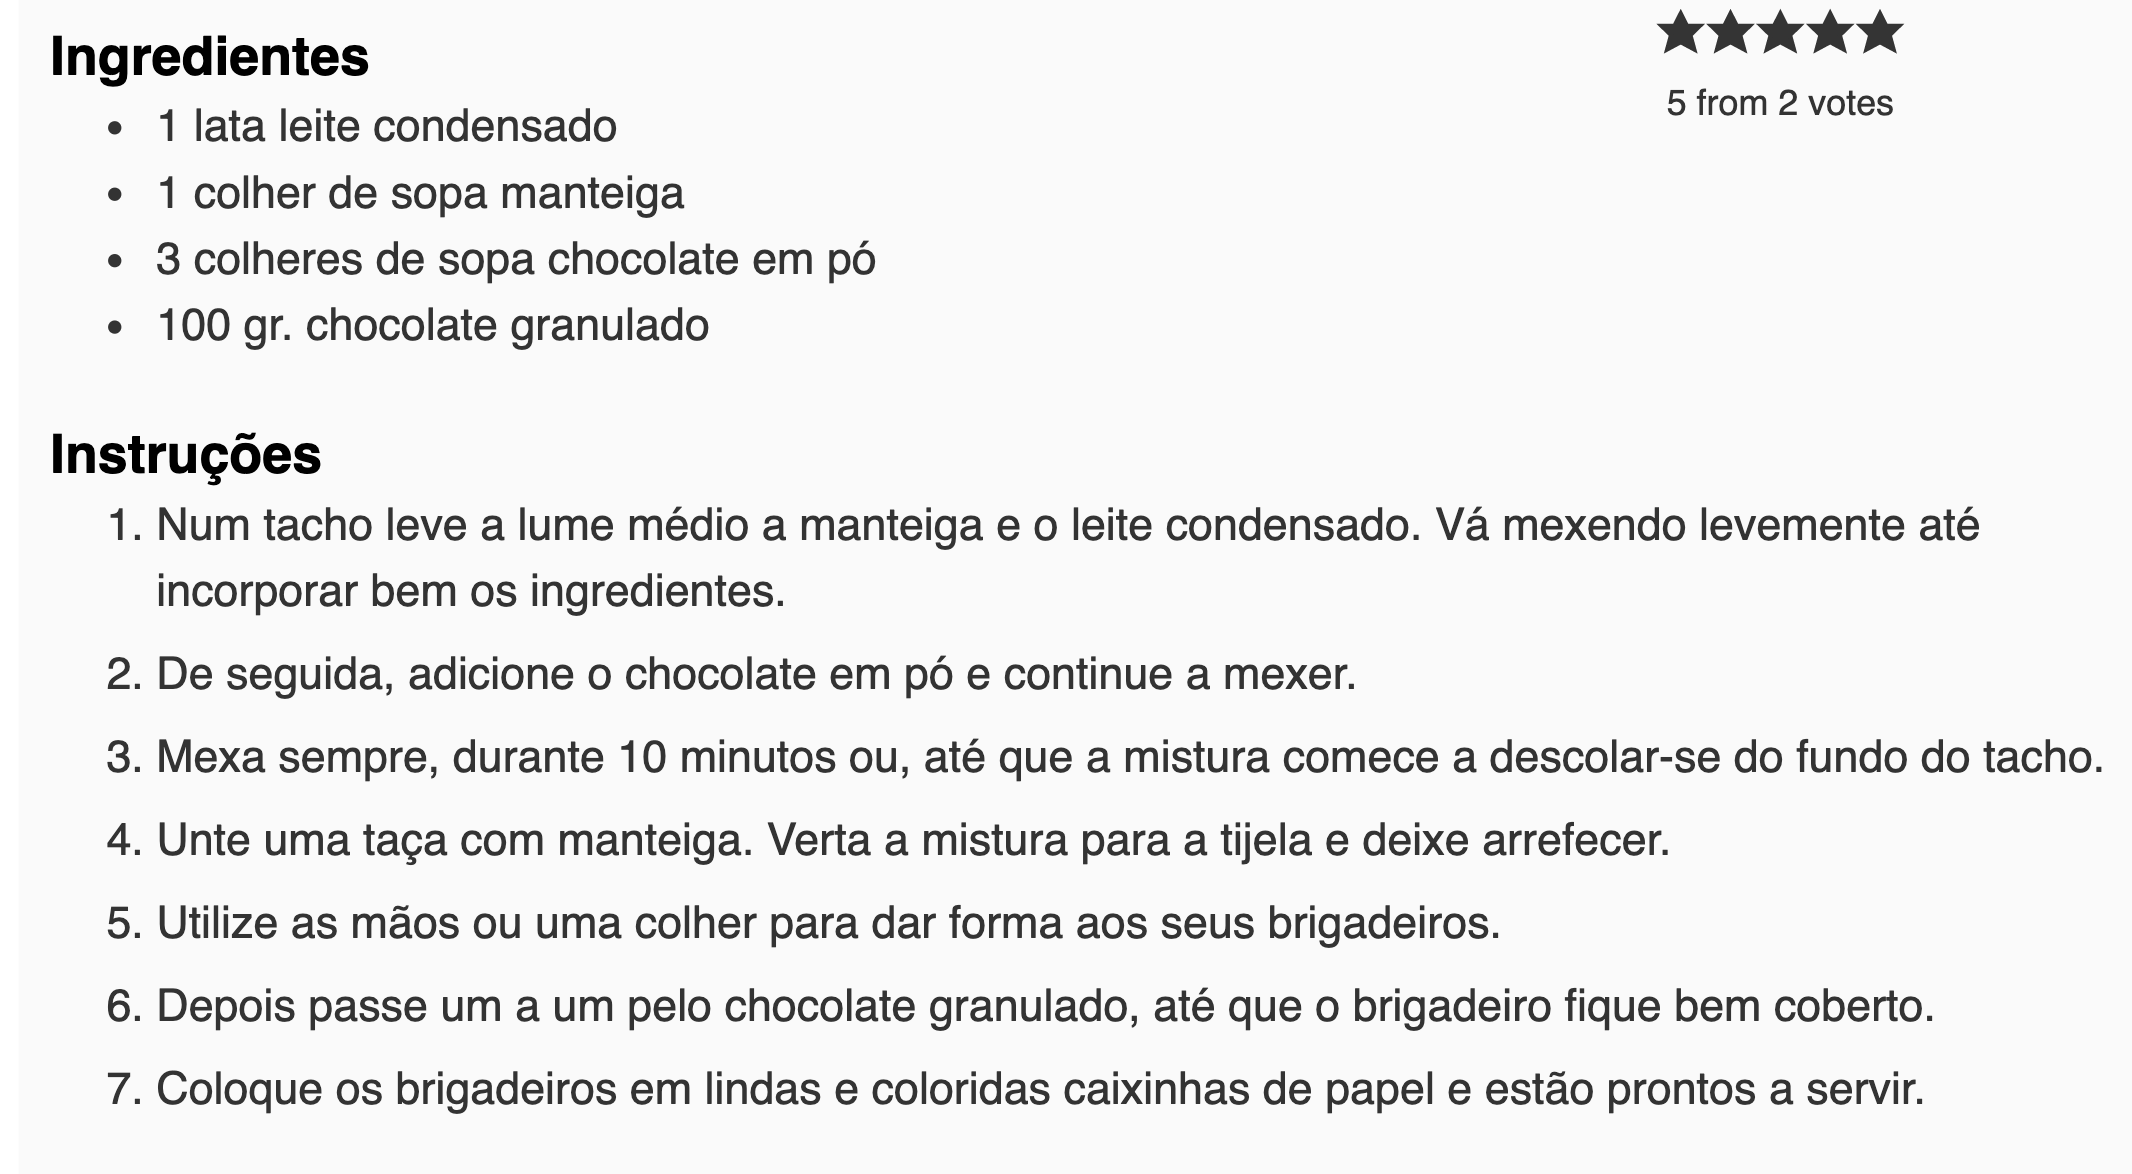
\includegraphics[scale=0.27]{figuras/Brigadeiro.png}
Entrada? Saída? Ações de processamento?
\end{frame}

\begin{frame}{Algoritmos e Programas}
\begin{itemize}
    \item \textbf{Algoritmo:} Descrição de passos para obter um resultado a partir de dados. 
    \\ \qquad (Descrição pode ser pouco rigorosa ou mais abstrata.)
    \item \textbf{Programa:} Implementação de um algoritmo.
    \\ \qquad (Descrição precisa, concreta a ser executada por 
    \\ \qquad \ um computador.)
    \item \textbf{Exemplos:}
    \begin{itemize}
        \item https://youtu.be/RoIY\_vEYglo \item \textit{Hello World} em C: 
        
        \qquad\qquad\qquad\qquad
        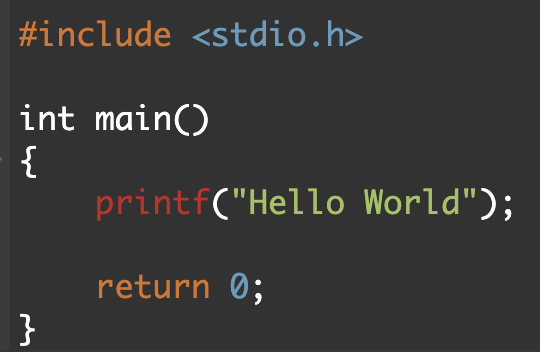
\includegraphics[scale=0.4]{figuras/helloworld.png}
    \end{itemize}
\end{itemize}
\end{frame}


\end{document}

% Introducao
%\section{Introdução}
\begin{frame}{Introdução}
	A Introdução vai aqui
\end{frame}

% Metodologia
\section{Metodologia}
\begin{frame}{Metodologia}
	Metodologia aqui.
\end{frame}

% Resultados
\section{Resultados}
\begin{frame}{Resultados}
	Resultados do trabalho  
\end{frame}


% Conclusao
\section{Conclusão}
\begin{frame}{Conclusão}
	Conclusões do trabalho  
\end{frame}

% Referencias
\section{Referencias}
\begin{frame}{Referências}
	Suas referencias bibliográficas aqui, siga o modelo ABNT.
	\bibliography{bib/bibliografia}
\end{frame}

% Agradecimentos
\section{}
\begin{frame}{Agradecimentos}
	Agradeço a todos. 	
\end{frame}

\end{document}